%!TEX root = ../template.tex
%%%%%%%%%%%%%%%%%%%%%%%%%%%%%%%%%%%%%%%%%%%%%%%%%%%%%%%%%%%%%%%%%%%%
%% chapter2.tex
%% NOVA thesis document file
%%
%% Chapter with the template manual
%%%%%%%%%%%%%%%%%%%%%%%%%%%%%%%%%%%%%%%%%%%%%%%%%%%%%%%%%%%%%%%%%%%%

\typeout{NT FILE chapter2.tex}%

\chapter{State-Of-The-Art}
\label{cha:State-Of-The-Art}

This chapter provides a view of the state-of-the-art of web development as well
as event management platforms and connection with iot devices.
Firstly, it presents an overview on how the web development is structured and
explains the concept of software architecture and some of its patterns. Then the
main two parts of web development, the frontend (both for web and mobile) and
backend, are discussed along with its frameworks.

In a second part, some event management platform solutions will be reviewed
along with its technologies.

Finally we will look on how we can connect a IoT device with our platform and
how its being already done in other solutions.

\section{System Architecture Patterns}

\subsection{Monolithic Architecture}
A monolithic architecture is a software design pattern in which all parts ---
such as the \gls{UI}, business logic and data access layers --- are tightly
coupled and deployed together as a single unit\cite{7436659,10031648}. This
was the most popular approach for decades due to how simple it is, specially in
the early stages of software development\cite{Garlan2018}.

\begin{figure}[htbp]
	\centering
	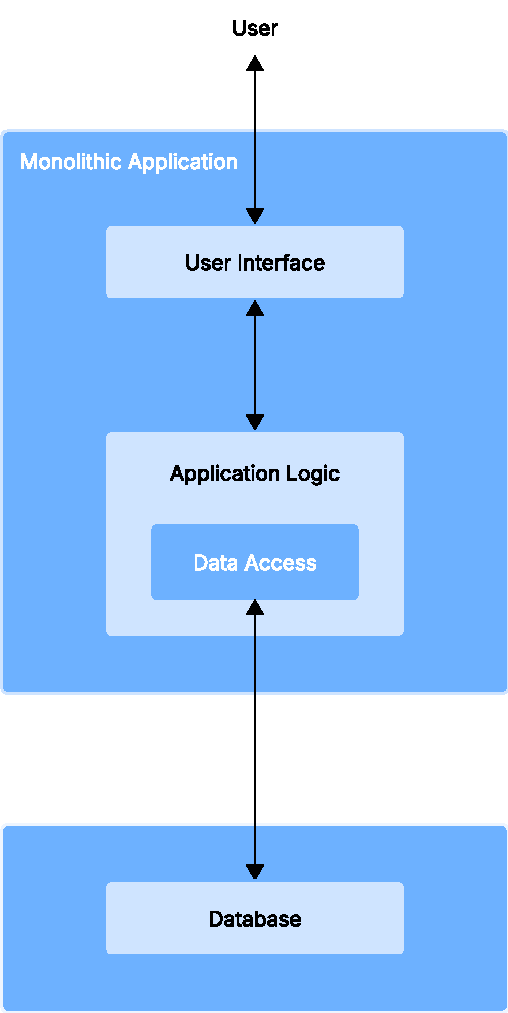
\includegraphics[width=0.8\textwidth, height=0.5\textheight, keepaspectratio]{Chapters/Figures/Architectures/Monolith.pdf}
	\caption{Monolithic architecture structure}
	\label{fig:architectures:monolithic}
\end{figure}

\subsubsection{Advantages}
Despite some problems, monoliths have some advantages on the other architectures,
specially for smaller applications or early-stage development:
\begin{itemize}
	\item \textbf{Simplicity}

	      The monolithic architecture is probably the simplest way of structuring a
	      project and monolithic solutions are easier to design, develop and deploy
	      than other solutions.
	      Having the code in a single codebase removes the need for complex
	      integration, making it more attractive for smaller teams with limited
	      resources or expertise.
	\item \textbf{Efficiency}

	      Since there is a single application in monolithic systems, there are no
	      services integrations and developers can debug without dealing with
	      inter-service communications. Testing is also easier because all of the
	      components are located in the same codebase and run in the same environment.
	\item \textbf{Straightforward Deployment}

	      Deploying a monolithic application involves managing a single artifact. This
	      reduces operational complexity compared to systems where deployment
	      pipelines must coordinate multiple services.
\end{itemize}
\subsubsection{Challenges}
For bigger architectures, this solution might not be adequate as several
challenges appear as applications grow in size and complexity.
\begin{itemize}
	\item \textbf{Scalability Constraints}

	      As mentioned above, Scaling a monolithic system can be much harder when
	      compared with other modular architectures. Let's say that hipotetically,
	      an application is composed of three modules. One is in constant
	      overload and needs to be scaled with urgency, the second has some peaks of
	      usage but doesn't require to be scaled, and the third is barely used and
	      could be ajusted to use less resources. In an architecture where this
	      modules are separated for example in three services, scaling publishers
	      efficient and we can scale up the first service and scale down the third.
	      However, in a monolith, we can only scale everything as one, meaning there
	      can be modules that force the scaling of unrelated components unnecesarily.
	      In the example above, we would need to scale the whole system, including
	      the third module that is already wasting more resources that it needs.
	\item \textbf{Maintenance}

	      Monoliths are prone to tech debt accumulation over time. The lack
	      of modularity present in these systems frequently results in what is known as a
	      "big ball of mud", meaning that dependencies between the system's elements are
	      unclear, slowing the development process and making maintenance an
	      hard and continuous process\cite{7333476}.

	\item \textbf{Deployment Risk}

	      Every change in the codebase requires all the application to be redeployed,
	      increasing the risk of downtime and complicating release cycles. If an error
	      is deployed to the public environment, it can cause the whole system to go
	      down while in modular systems, if a problem is deployed in one of the
	      modules, the others are independent and can still run even if the one with
	      the problem is down, meaning that only part of the system is unavailable.

	\item \textbf{Lack of Flexibility}

	      Since all of the application's logic resides in a single codebase, it will
	      likely be enforced that everything should be developed using an uniform
	      technology stack. In architectures that have the application divided in
	      modules is possible for each module to have its own technology stack,
	      which can facilitate the development of some specific features that are
	      easier to do with specific technologies.
\end{itemize}

\subsection{Client-Server Architecture}
The client-server architecture is a software design paradigm that devides the
system into two types, the clients and the servers. The clients are service
requesters responsible for initiating requests tipically as consequence of user
interaction, and can be for example a website or a mobile app. On the other
side, servers process that requests, access the data if needed and return the
adequate responses. This separation of concerns allows one server to provide
consistent data to multiple clients.
Examples include email systems, where clients(e.g. email software) interact with
a centralized server that is responsible for sending and storing the emails.

\begin{figure}[htbp]
	\centering
	\includegraphics[width=\textwidth, height=0.5\textheight, keepaspectratio]{Chapters/Figures/Architectures/Client-server.pdf}
	\caption{Client-Server architecture structure}
	\label{fig:architectures:client-server}
\end{figure}

\subsubsection{Advantages}
The client-side architecture has several benefits:
\begin{itemize}
	\item \textbf{Modularity}

	      A separation between clients and servers allows for independent development,
	      testing and maintenance, improving flexibility in application design.

	\item \textbf{Data Consistency}

	      Multiple clients can access a single server, and since this server is the
	      only thing managing the resources it ensures that the data received by the
	      clients is consistent between them. This also ensures that clients can access
	      the most recent and accurate information.

	\item \textbf{Scalability}

	      Horizontal scaling, where additional servers can be added, altought limited
	      by replication of the entire server, enables the system to handle increased
	      demand.
\end{itemize}
\subsubsection{Challenges}
The Client-Server Architecture has also its disadvantages:
\begin{itemize}
	\item \textbf{Single Point of Failure}

	      All the resources are managed in a centralized server, which means that if
	      the server fails, all connected clients are affected. Despite this being a
	      serious concern, there are techniques like load balancing that help
	      mitigating this risk.

	\item \textbf{Scalability Constraints}

	      Although scalability was mentioned above as an advantage, the scalability
	      of client-server achitectures is very limited. Even with the decoupling of
	      clients from servers, horizontal scaling can only happen by deploying the
	      same server to several machines and vertical scaling can only happen by
	      increasing the hardware for the whole server. This is limited in modularity
	      and it also increases the complexity by adding the necessity of having
	      load balancers and data synchronization across servers.

	\item \textbf{Latency}

	      Communication between clients and servers over a network introduce delays,
	      which can be a problem for applications that require real-time
	      responses.

\end{itemize}

\subsection{Microservices Architecture}
The microservices architecture is a system design pattern that divides an
application into several other independently deployed applications called
microservices.
In this solution, the modules communicate between each other through
synchronous communications using APIs based on technologies like like
\gls{HTTP}, \gls{gRPC}, or GraphQL, or through asynchronous communication,
adopting tools like message brokers or event streaming platforms.

\begin{figure}[htbp]
	\centering
	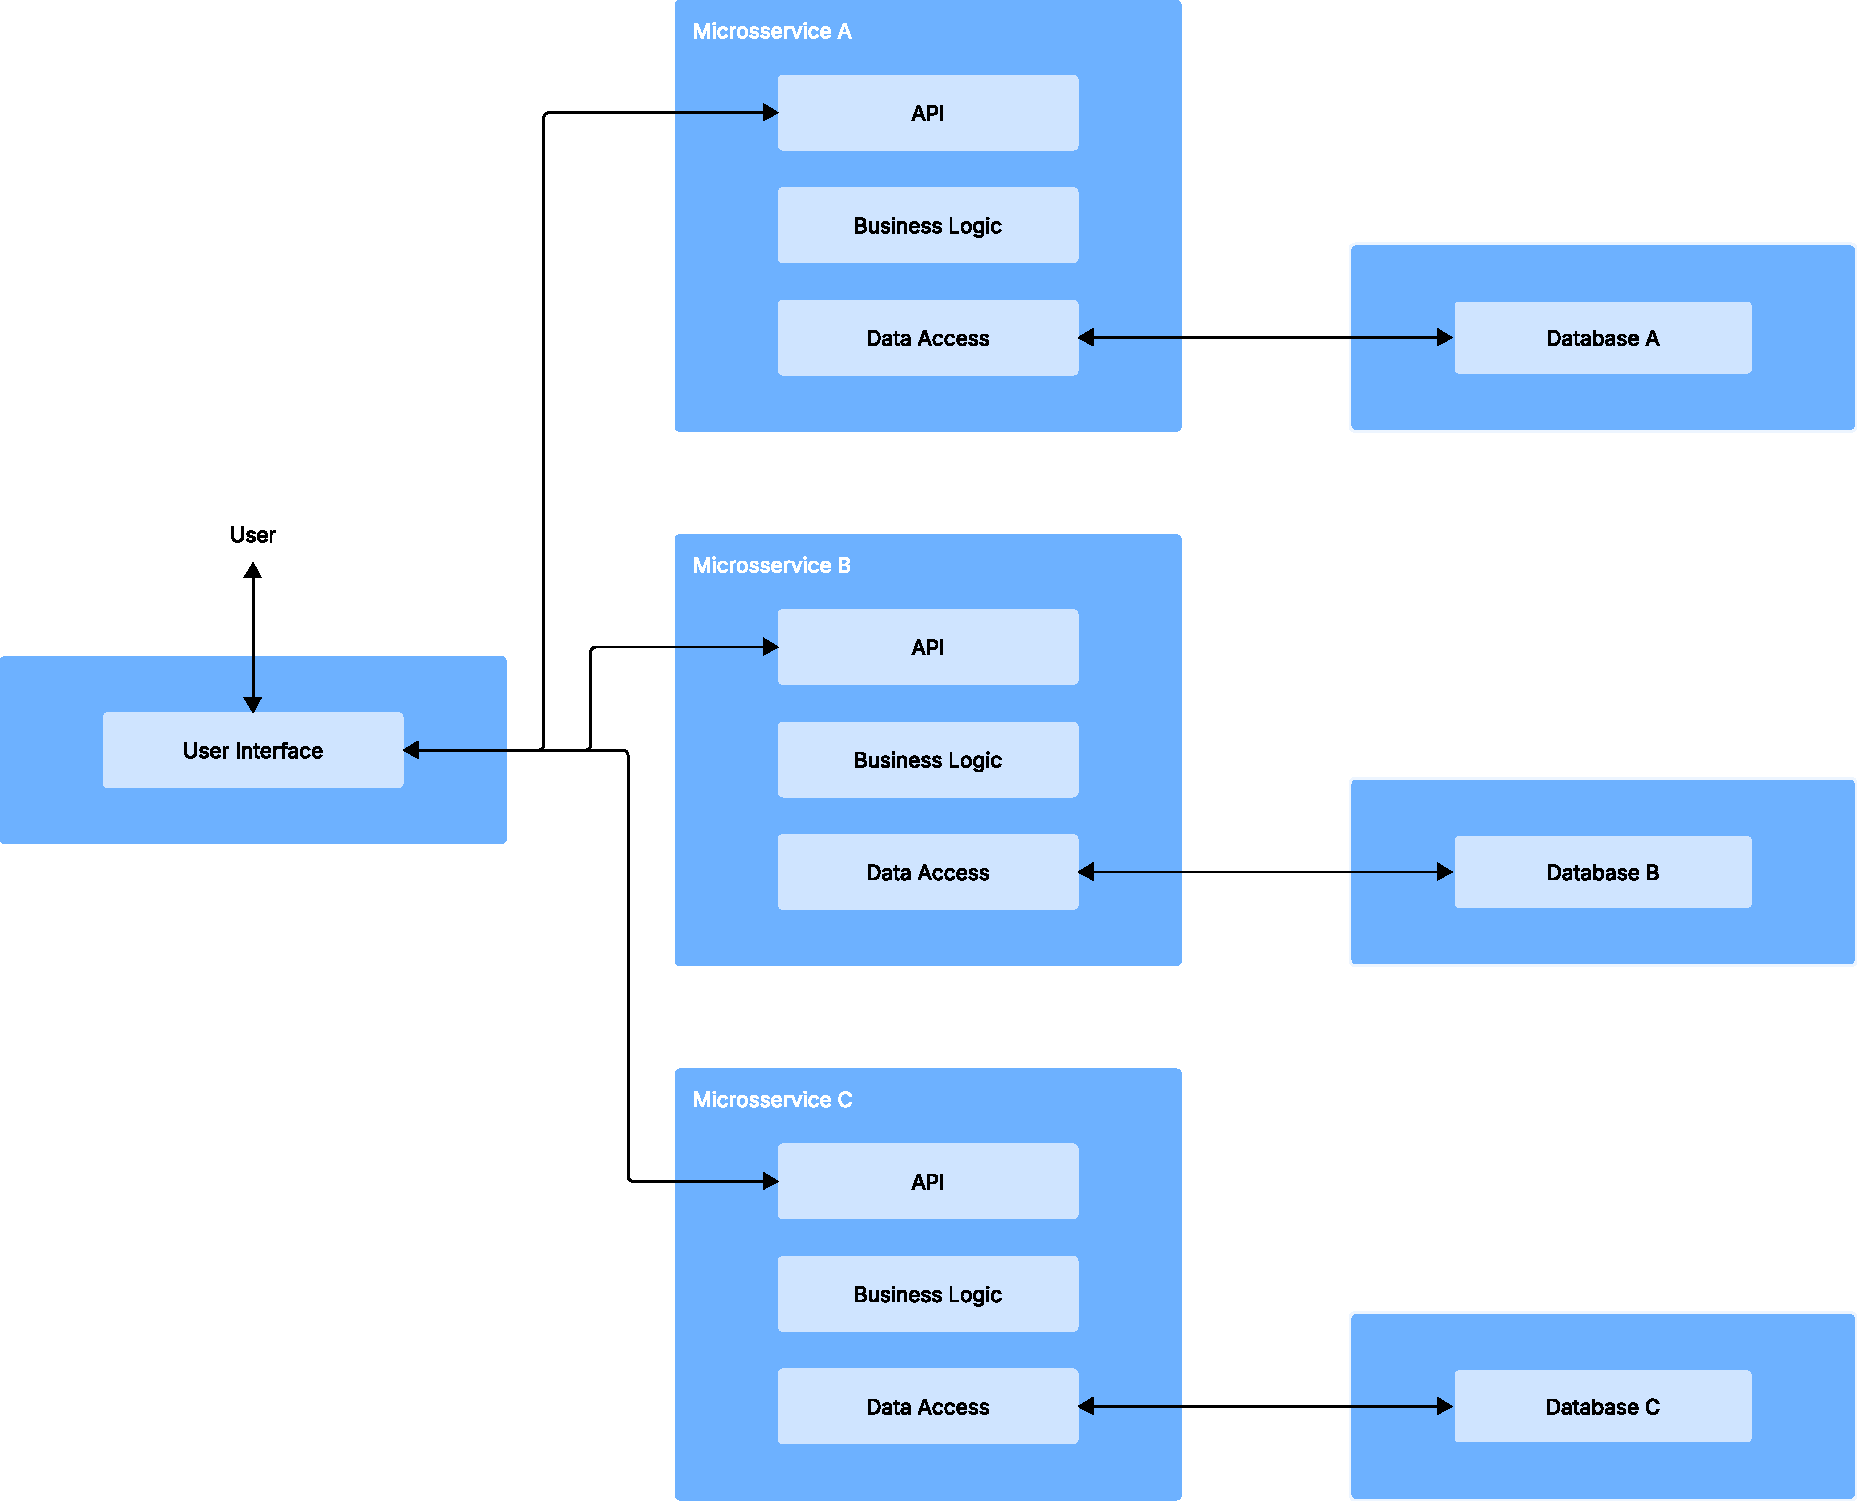
\includegraphics[width=\textwidth, height=0.5\textheight, keepaspectratio]{Chapters/Figures/Architectures/microservices.pdf}
	\caption{Microservices architecture structure}
	\label{fig:architectures:microservices}
\end{figure}

\subsubsection{Advantages}

\begin{itemize}
	\item \textbf{Scalability}

	      Microservices are independent applications with its own codebase, deployed
	      separately and in most cases with their individual database. For this reason
	      each service can be scaled independently based on demand. A service with
	      high demand like for example user authentication can scale separately from
	      services with less workload.

	\item \textbf{Fault Isolation}

	      Another benefit of having the logic separated into services is that when
	      a failure occurs in a service, the others will unlikely be affected. For
	      example, when a store website has a problem with its payment service, the
	      users might not be able to pay but they can still browse the website and
	      do other things like managing the profile or adding products to the cart.

	\item \textbf{Technology Diversity}

	      Each service is an independent application, which means that each service
	      can be developed using different technologies. This allows the service to
	      be developed using technologies that are more suitable for its own purpose.

\end{itemize}

\subsubsection{Challenges}
\begin{itemize}
	\item \textbf{Complexity}

	      Managing multiple services is much more complex than managing a single
	      application. Deployment and maintenance efforts are multiplied, which can
	      lead to operational overhead. The heavy use of monitoring tools can be
	      helpful, or even required in this kind of solutions.

	\item \textbf{Dependency Management}

	      In these architectures, services often depend on each other, and despite
	      fault isolation being pointed as an advantage, if the dependencies are not
	      properly managed a failure can lead to successive failures on other modules.
	      When there are two services that need to be change in order to add or update
	      a feature, the first service to be deployed need to be compatible with the
	      previous version of the other, otherwise there will be problems while they
	      are not both properly deployed.
	      Observability tools like tracing and logging are essencial to prevent and
	      diagnose this king of issues.
\end{itemize}


\subsection{Event-Driven Architecture}
The event-driven architecture is a system design patter where the components
are loosed coupled, communicating by events. Events are messages that are sent
by a system in reaction to a change in its state. This communication is made
between an event producer, and an event subscriber. Event Producers generate the
events and send the messages to a broker, Event Subscribers subscribe to
events and react to them. Both these parts are agnostic to each other, meaning
that the producers send the events not knowing who will receive them and the
subscribers receive the events not knowing who sent them. This is possible
because of the broker. Event Brokers, like Apache Kafka or RabbitMQ are
responsible for routing the events from the producers to the subscribers through
features like message queuing and topic-based routing.

\begin{figure}[htbp]
	\centering
	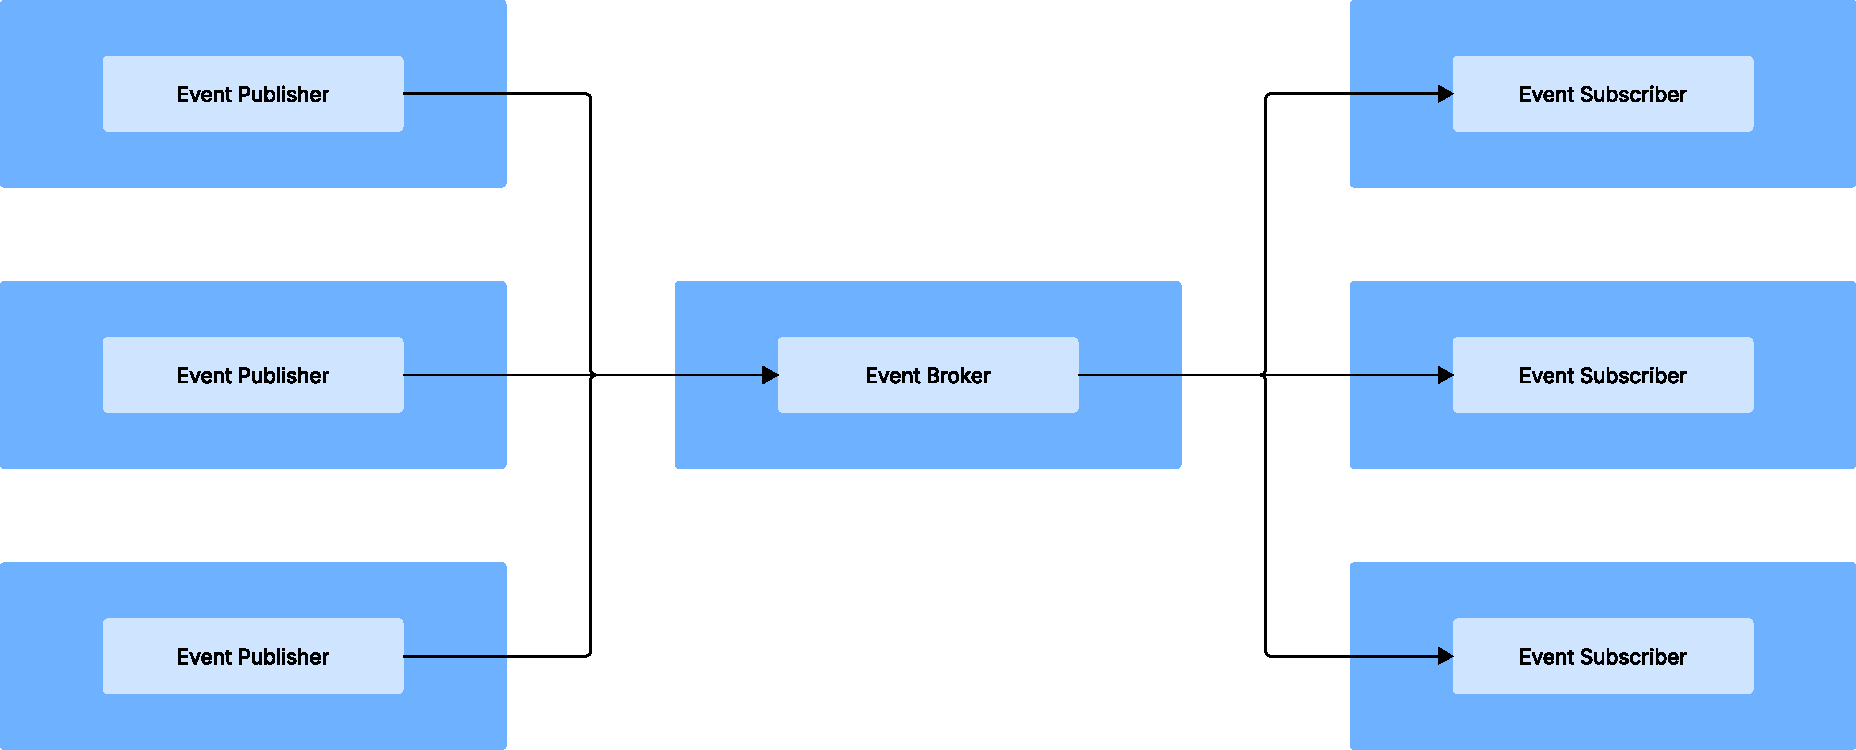
\includegraphics[width=\textwidth, height=0.5\textheight, keepaspectratio]{Chapters/Figures/Architectures/Event-driven.pdf}
	\caption{Event-driven architecture structure}
	\label{fig:architectures:event-driven}
\end{figure}

\subsubsection{Advantages}
\begin{itemize}
	\item \textbf{Loose Coupling}

	      The communication is done indirectly, reducing the interdependencies which
	      are a significant point of failure.

	\item \textbf{Scaling}

	      Since the communication can be done asynchronously and through event brokers,
	      the events don't need to be processed in real-time and are instead added to
	      a queue allowing these systems to support an high volume of events. This
	      reduces the needing for scaling, which is already an easier process because
	      of the modularity present in this architecture.

	\item \textbf{Fault Tolerance}

	      Components of an event-driven architecture operate independently, meaning
	      that if a component fails the system can continue functioning. In this
	      case, due to the existence of an event broker, the messages are stored in
	      this intermediary until they are processed, reducing the probability of
	      loosing data.

	\item \textbf{Flexibility in adding features}

	      By decoupling producers from subscribers, a new consumer can be added
	      and subscribe to existing events. This doesn't require any change in the
	      producer in order to work, which facilitates the extension of the
	      system.

	\item \textbf{Real-Time capabilities}

	      Despite what was said above that the events don't need to be processed
	      in real-time, they can be configured to process and respond to events
	      as they occur, making it ideal for applications which require real-time
	      responsiveness.
\end{itemize}

\subsubsection{Challenges}
\begin{itemize}
	\item \textbf{Event Ordering and Duplication}

	      Making sure that events are queued in the correct order and that they are
	      processed only once can be a difficult task because of the concurrency
	      that is characteristic of these systems.

	\item \textbf{Debugging}

	      The assynchronous communication complicates the debugging process.
	      Observability tool are essencial to diagnose problems.

	\item \textbf{Infrastructure Overhead}

	      The process of setting up and maintaining the event brokers, monitoring
	      systems introduce complexity on the operational side.
\end{itemize}

\subsection{Serverless Architecture}
Serverless architecture is a solution where the cloud provider manages all the
server infrastructure, scaling, and maintaining it automatically as needed.
Serverless applications are made of event-driven stateless functions that run
only when needed. This functions are triggered through events like API calls,
database changes, message queues or IoT events and shutdown after execution,
making this a highly efficient solution.

\begin{figure}[htbp]
	\centering
	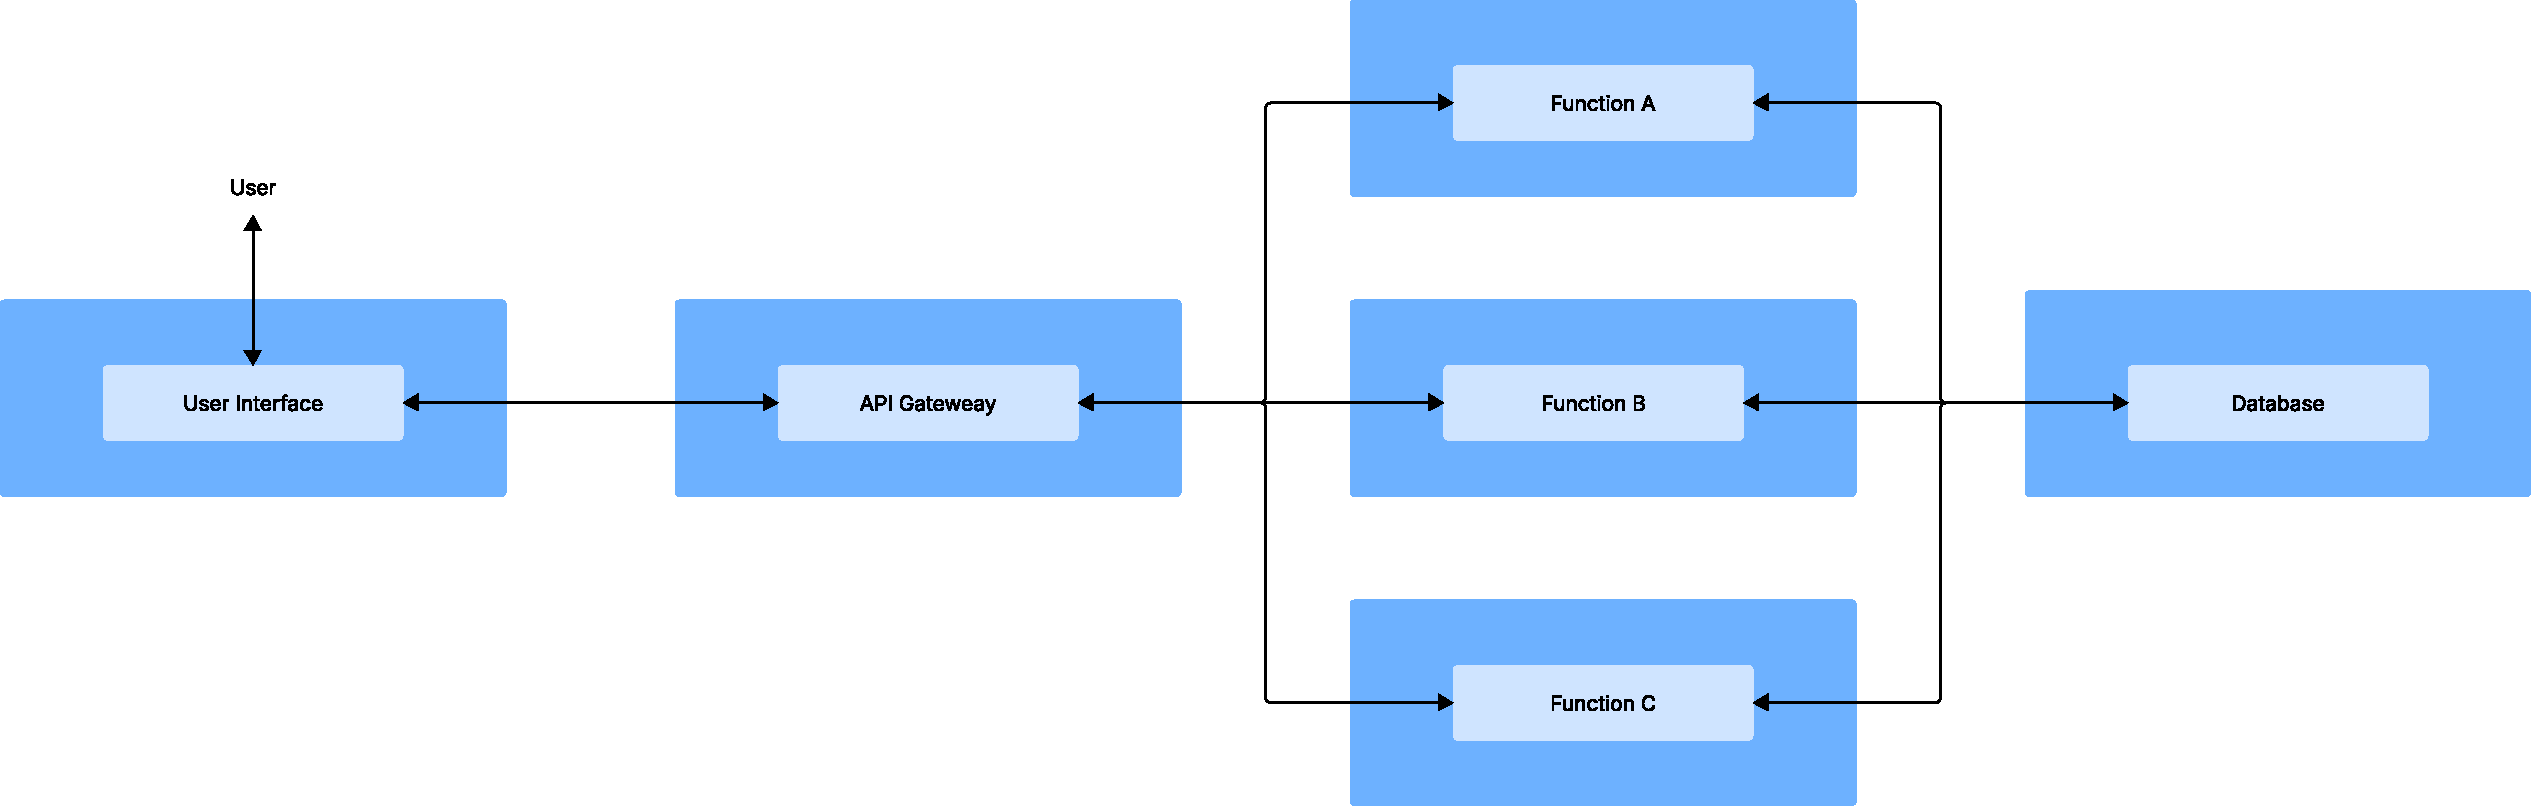
\includegraphics[width=\textwidth, height=0.5\textheight, keepaspectratio]{Chapters/Figures/Architectures/Serverless.pdf}
	\caption{Serverless architecture structure}
	\label{fig:architectures:serverless}
\end{figure}

\subsubsection{Advantages}
\begin{itemize}

	\item \textbf{Scalability}

	      The application automatically scales horizontally as needed, creating or
	      deleting function instances in response to demand. This is a great
	      advantage for applications with peak times where the demand is
	      significantly bigger than normal.

	\item \textbf{Cost Effective}

	      Unlike servers, that are usually paid by uptime, serverless functions are
	      tipically paid per execution, reducing costs when the application is idle.

	\item \textbf{Focus on Development}

	      Since the developers don't need to handle all the infrastructure management,
	      they can focus entirely on the code, usually resulting in improvements in
	      produtivity and code quality.


\end{itemize}

\subsubsection{Challenges}
\begin{itemize}
	\item \textbf{Cold Start}

	      After a long period of inactivity, functions take longer to execute, which
	      can be a problem for applications that require real-time responsiveness.

	\item \textbf{Execution limits}

	      Serverless cloud providers usually have execution time limits. AWS lambda,
	      for example, has a 15 minute execution time limit, making this solution
	      not reliable for long running functions.

	\item \textbf{Testing and Debugging}

	      Testing and debugging in serverless architectures are harder due to the
	      decentralized nature of this systems.

	\item \textbf{Statelessness}

	      Functions can not store data between executions and due to that, some
	      applications will require external storage solutions.
\end{itemize}

\subsection{Edge Architecture}
Edge architectur is a system design pattern in where the data is processed
closer to where it is generated. This practice is called edge computing and
is commonly used in IoT systems, with data being process in the device
before being sent to a server.

\begin{figure}[H]
	\centering
	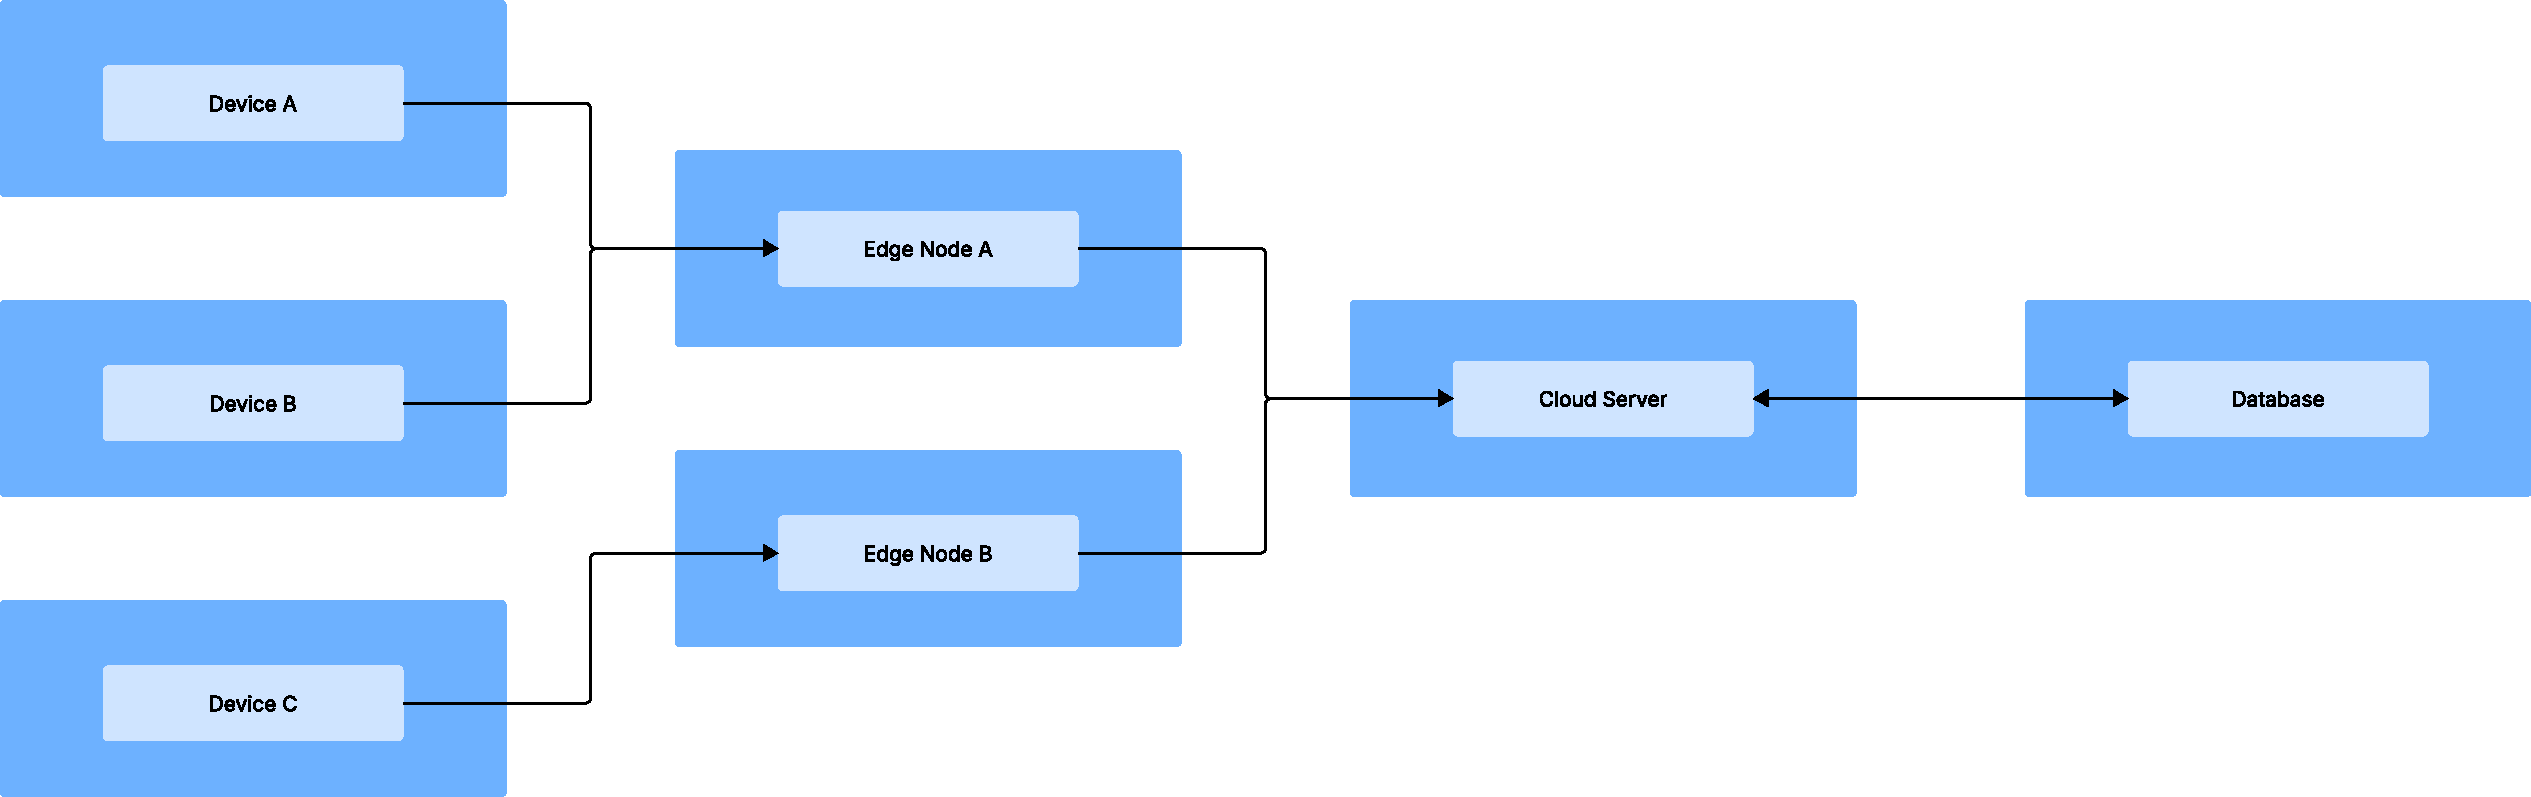
\includegraphics[width=\textwidth, height=0.5\textheight, keepaspectratio]{Chapters/Figures/Architectures/Edge.pdf}
	\caption{Edge architecture structure}
	\label{fig:architectures:edge}
\end{figure}

\subsubsection{Advantages}

\begin{itemize}


	\item \textbf{Low Latency and Bandwidth}

	      Since there's no need to access a server, it allows for real-time decisions
	      in systems like self-driving cars or industrial automation. When there's
	      still data being sent to a server, the data can be processed and filtered
	      locally before being sent, reducing bandwidth usage.


	\item \textbf{Reliability}

	      It can operate offline by storing data locally until the connection is
	      restored.

	\item \textbf{Data Privacy}

	      Sensitive data, like someone's biometric data can be kept in the device,
	      instead of being transmitted to the cloud.

\end{itemize}

\subsubsection{Challenges}
\begin{itemize}

	\item \textbf{Limited Resources}

	      Edge devices are usually constrained in processing power and storage capacity.

	\item \textbf{Security Risks}

	      Edge devices are more vulnerable to attacks, both physical and cyberattacks.

\end{itemize}

\subsection{Applications and Use Cases}
Every architecture has its own advantages and disadvantages, but they all have
their place in the software industry.

Monolithic systems are a great choice for simpler and smaller applications.
Startups and small businesses usually start by implementing this solution as
its infrastructure is very simple, and it's relatively fast to have an initial
functional product. This architecture is often used as a starting point, and
eventually, as the application grows, it's migrated to more complex architectures.
Examples of real-world applications are basic e-commerce platforms, content
management systems and small desktop applications.

The client-side architecture is popular among web applications. Most of the
websites use this architecture where browsers act as clients that interact with
centralized web servers. Another wide applicatios for this structures are email
systems and database applications. In email systems, the servers communicate
with clients like Microsoft Outlook or Gmail using protocols like IMAP or SMTP.
In database applications, clients access centralized database servers using
SQL queries for data retrieval and manipulation.

Microservices architectures have become the go-to solution for more complex
systems. It's widely used in bigger e-commerce applications where the application
is divided into several microservices like user authentication, payment processing,
shipping processing, etc. Streaming platforms like Netflix also tend to use this
solution, dividing the application into services for content recommendation, user
preferences, subscription handling, etc.

Lastly, the event-driven architecture shines in products where real-time
responsiveness is crucial. It's widely used in Internet of Things systems,in
applications like industrial monitoring, home automation, and environmental
sensing where IoT devices send events to be processed in real-time.

It's also common to mix different architectures in the same system using
hybrid solutions. E-commerce platforms, for example, where referenced above in
multiple architectures as these platforms can use microsservices for processing
payments or user authentication and event-driven architecture to process orders.

\section{Backend Development}
Managing the underlying logic, data storage, and communication processes that
allow the web application to operate is the responsibility of the backend.
The backend operates behind the scenes managing data, processes requests, and
responding to them, while the frontend gives users a visual and interactive
experience. E-commerce platforms can also use event-driven architecture for
features like processing orders or updating inventory.

\subsection{Backend Frameworks}
\subsubsection{Express}
Express is a minimalist and lightweight web application framework for Node.js,
designed to simplify server-side development. It's characterized by being
fast and unopinionated, which means that it is flexible in the way you implement
things.
In Express, it's possible to stack functions (middlewares) to handle \gls{HTTP}
requests sequentially, allowing custom logic to be easily integrated.
Routing using this framework is straightforward. It's very simple to define
paths and associate handlers. On top of that, Express allows the grouping of
routes into distinct modules, improving code organization.
Although this framework is mostly seen as a backend solution, it supports
integration with various template engines like EJS, Pug, and Handlebars,
providing a way to render dynamic HTML pages.
Despite having a simple and clean approach to the development of RESTful APIs,
this framework lacks built-in features. Express doen't provide features like
dependency injection, user authentication, database integration or input
validation which all need to be implemented using third-party libraries.
By being an unopinionated solution, it lacks structure, increasing the effort
of the developers on manually configuring middlewares, and maintaining the code
organized, specially for more complex projects.
Express is a popular framework, being adopted by many developers. Resources
about this technology, like documentation or tutorials are easy to find
everywhere, due to its vast community, which might be an advantage for
developers less experienced.

\subsubsection{Nestjs}
Nest JS is an opinionated Node.js framework with a highly structured
development environment. It has a very rich environment providing many built-in
features.

With Typescript support, NestJS ensures strong typing, reducing the risk of
having runtime errors.

This framework simplifies the process of building applications with
microservices or event-driven architectures by providing native support for
communication technologies like GraphQL, and websockets, and easy configuration
for technologies like RabitMQ, MQTT, Kafka and \gls{gRPC}.

NestJS integrates a powerful dependency injection system, which, apart from the
increase in performance, also helps the developers writing clean code, testing,
and maintaining it.

Applications in Nestjs are divided into
self-contained modules, making large applications easier to scale and maintain.

On the other side, due to the structured and opinionated approach, the learning
curve might be steeper than other simple solutions like Express.
It has also the disadvantage of being a heavier framework, slightly loosing
performance. This performance overhead is usually imperceptible in most
applications.

Due to its structured approach, it can be a great choice for more complex
applications, specially applications with microservices or event-driven
architectures.
\subsubsection{Java Spring}
Spring is a the most popular framework for building complex and robust
applications using Java. It's a great solution for developing scalable and secure
applications. It's one of the most complete backend frameworks having features
like dependency injection, and extensions for developing REST APIs and
microservices.

A popular extension for Spring is called Spring Boot and its job is to
simplify configuration and deployment. It provides opinionated defaults,
reducing boilerplate code and improving development speed.

Another popular extensions include Spring MVC for building RESTful APIs, Spring
Cloud for building microservices and Spring Security for implemenenting
security features like authentication and authorization.

Spring also includes suport for testing tools like JUnit and Mockito.

Applications developed in spring are easily scalable due to Spring's modular
design.
It's a very flexible solution handling every type of architectures, from
monoliths to microservices.

On the other side, just like NestJS, Spring has a steeper learning curve when
compared to more simple and straightforward solutions. Learging concepts like
dependency injection or Inversion of Control can be overwhelming for less
experienced developers.
On top of that, configuring Spring is a complex task that requires significant
boilerplade code and XML configuration. This effort can be reduced with Spring
Boot.
Another downside of this framework, is that it's an heavy framework and
requires higher resources to run when compared with other lightweight solutions.

\subsubsection{Flask}
Flask is a simple, lightweight and flexible framework for Python. It's a
minimalist framework, providing only the essencial features needed for
web development, leaving the more complex ones for extensions. It has the basic
features like a straightforward routing process, request handling and Jinja2,
a built-in template engine. Apart from this essencial structure, Flask has a
rich ecossystem of extensions, providing features like authentication,
database access and input validation.

Although the advantages are clear, there are also some challenges. Scaling
Flask applications for high traffic usually requires additional tools like load
balancers and asynchronous task queues. As refered above, another clear
drawback is the lack of built-in features. Lastly, the unopinionated nature and
flexibility provided by this framework can lead to inconsistent implementations
of the same features across a single project, with different developers using
different tools or patterns.

Despite this possible disadvantages, Flask is still a good choice for small to
medium sized applications.

\subsubsection{ASP.NET Core}
ASP.NET Core is an open-source framework developed and maintained by Microsoft.
It's a high-performance framework designed for scalability and modularity and
widely used for developing complex web applications.

Contrary to all the other frameworks mentioned above, this framework can be
used with more than one programming language. C\# is the most used language, but
the developers can also choose between F\# and Visual Basic, the last with some
limitations.

This framework was designed with performance in mind, and some benchmarks show
it as one of the fastest backend frameworks available.

ASP.NET Core provides features like dependency injection and includes tools for
authentication and authorization, supporting common protocols like JWT or OAuth.
It also includes other security features like prevention against cross-site
scripting attacks or data protection.

Despite being mainly a backend framework, its also possible to develop the
frontend using this framework. Features like Razor Pages, MVC or Blazor allow
some limited frontend capabilities.

ASP.NET Core implements a modular midleware pipeline that processes HTTP
requests which developers can configure to include middlewares for tasks like
authentication, authorization, logging and error handling.

Despite all the good things about this framework, there are also some drawbacks.

Like another frameworks already mentioned, developers that are new to this
technology may also face a steep learning curve, mainly regarding advanced
features like dependency injection and middleware pipelines.

Setting up the middleware pipeline and dependency injection can be a complex
process.

This framework can be a great choice for large-scale systems, but overwhelming
for smaller projects.
\subsubsection{Laravel}
Laravel is a popular PHP framework built using the Model-View-Controller
pattern. It's a simple but complete framework offering a great set of built-in
tools. It includes an Object-Relational Mapping tool called Eloquent, and a
template engine called Blade. It also provides built-in tools for tasks like
authentication, authorization, task scheduling, and testing. Lastly, it
provides protection against security vulnerabilities such as SQL injection,
cross-site scripting and cross-site request forgery attacks.

Some advantages of this framework include an increase in development
productivity, a rich ecosystem, scalability, and security.
By having an expressive syntax and great documentation, Laravel enhances
development productivity, reducing development time.
Laravel has an extensive ecosystem, having tools like Laravel Forge for server
management, Laravel Nova for admin panel development and Laravel Vapor for
serverless deployment.
Applications written with this technology can usually scale both horizontally
and vertically with ease, using tools like queues and caching, making this
framework suitable for both small and large projects.

On the downside, Laravel trades its completeness by performance, having a
lower performance when compared with more lightweight frameworks.
Altought this framework can suite large projects, it requires complex
optimization with tools like caching, load balancing and database tuning.
Despite being a simple framework it has a steep learning curve because of its
specific tools and it's also a framework that's very dependent on its plugins,
which can be a problem, since the developers can't control the quality of the
plugins, and its issues may become issues for the application.

\section{Communication and Security}
Both communication and security are very important parts of any system.
Deciding which protocols should be used or how to address security concerns are
important parts of designing a software system. In the context of this
dissertation, we need to address both communication between IoT systems and
Backend, and Frontend and Backend.


\subsection{Communication between IoT systems and backend}
IoT devices collect data that is then sent to backend services to be processed
and analyzed. This often requires low-latency and reliable communication.
\subsubsection{Communication Protocols and Standards}
There are many protocols that address the necessities of IoT systems:

\begin{itemize}

	\item \textbf{MQTT}

	      MQTT is a lightweight bi-directional message protocol created in 1999.
	      It follows the publisher-subscriber architecture decoupling the message
	      sender from the receiver. This protocol is composed by two parts, the
	      broker, and the clients. The broker is the system responsible for providing
	      a safe transmittion between clients implementing authentication and
	      authorization features and routing the messages from the publishers to
	      the respective subscribers. The clients are every application that
	      communicates with the broker, being either a publisher or a subscriber.
	      It's commonly used in resource-constrained systems like IoT systems because
	      it's easy to implement and requires low bandwidth.

	\item \textbf{AMQP}

	      AMQP is another message protocol just like MQTT.
	      Despite being similar this protocols have some differences. While MQTT is
	      focused on simplicity and low-bandwidth communication, AMQP is optimized for
	      more complex systems, providing robust and reliable message queuing and
	      routing introducing concepts like exchanges and queues.


	\item \textbf{CoAP}

	      CoAP is a HTTP based protocol optimized for resource-constrained
	      environments, such as IoT systems. It's built on UDP instead of TCP,
	      resulting in a lightweight and faster solution.
	      This protocol follows the RESTful design providing resources under a URL
	      using methods like GET, POST, PUT, and DELETE. Due to its similarity with
	      HTTP, one of the most widely used protocols, CoAP can be easily integrated
	      with HTTP using proxys.

\end{itemize}

\subsubsection{Middlewares and Gateways}
Middleware platforms and gateways can be used in IoT-to-backend
communication to simplify the device integration and improving scalability:

\begin{itemize}

	\item \textbf{Middlewares}

	      Platforms like AWS IoT Core or Google Cloud IoT have features like
	      device management, protocol translation, and analytics in real-time that
	      can be usefull when integrating IoT systems with backend services.

	\item \textbf{Gateways}

	      Gateways are platforms that can aggregate, preprocess and filter data
	      from IoT systems. This way, only usefull data is sent to the backend server,
	      removing useless,resource consuming interactions.

\end{itemize}

\subsection{Communication between Frontend and Backend}
Backend is where all the business logic relies and it's what provides frontend
the data for it to display to the end user. An effective communication between
these two parts is crucial for a well designed system.
\subsubsection{Protocols}
An API is an interface of an application that defines a set of rules and
protocols that allows other applications to communicate with it. There are many
protocols that can be used to transmit data, some examples are:

\begin{itemize}

	\item \textbf{HTTP/HTTPS}

	      HTTP is the most widely used protocol for APIs. It works on a
	      request-response model, where the client sends the request and the server
	      responds. It's a stateless, meaning each request is independent and doesn't
	      affect the others. It's commonly used for fetching HTML, images, videos
	      and other resources over the internet. HTTPS is the same as HTTP but the
	      data is encrypted using TLS or SSL.


	\item \textbf{WebSocket}

	      WebSocket is a protocol designed for real-time bi-directional communication.
	      It operates over TCP and starts as an HTTP connect and then changes to a
	      WebSocket connection. Unlike HTTP it doesn't rely on requests, and both
	      parts can communicate at any time.


	\item \textbf{UDP/TCP}

	      TCP is a connection-oriented protocol that ensures reliability by
	      estabilishing a connection via a three-way handshake, retrying lost
	      packets and ensuring data is received in the correct order.
	      On the other side UDP is a connectionless protocol which sends data in
	      independent packets. It doesn't guarantee delivery, order or error
	      correction. Because of this, UDP is faster but less reliable.


\end{itemize}


These protocols define rules for communication between systems, focusing on the
technical implementation. On a higher level are the APIs.
The APIs define how data is requested, sent and consumed.

\begin{itemize}
	\item \textbf{REST}

	      RESTful APIs are APIs that follow the REST principles. This APIs'
	      communication are stateless, meaning that each request must have all
	      the information required for being processed.
	      REST APIs provide resources through unique URLs associated to them, and
	      each resource idependent meaning that it doesn't depend on other
	      requests. The transport protocol used by these APIs is HTTP or HTTPS.

	\item \textbf{GraphQL}

	      GraphQL allows clients to specify exactly the data they need. This
	      flexibility avoids over-fetching(getting more data than necessary) and
	      under-fetching (not getting enough data in a single request).
	      Just like RESTful APIs, GraphQL works with HTTP or HTTPS but GraphQL APIs
	      usually expose a single HTTP endpoing for all requests.
	      GraphQL supports subscriptions, which allows the client to receive
	      real-time updates.

	\item \textbf{gRPC}

	      gRPC was developed by google and can be seen as both a protocol and an
	      API style. With this protocol, both clients and servers can call
	      functions on each other, just like if it was its own code.
	      It's commonly used in microservices architectures and real-time applications.

	\item \textbf{SOAP}

	      Despite SOAP being defined as a protocol, it's more comparable to API
	      types since it runs on top of transport protocols like HTTP, TCP or
	      SMTP(email).
	      SOAP is a lightweight protocol for exchanging structured data. It uses XML
	      to format messages in its own standards. These strict standards ensure
	      reliability and compatibility between systems.

\end{itemize}
\subsection{Security}

Security is a crucial part of any system, it ensures the integrity of both
the data and the system. When projecting the security in a system some
aspects need to be addressed:

\begin{figure}[htbp]
	\centering
	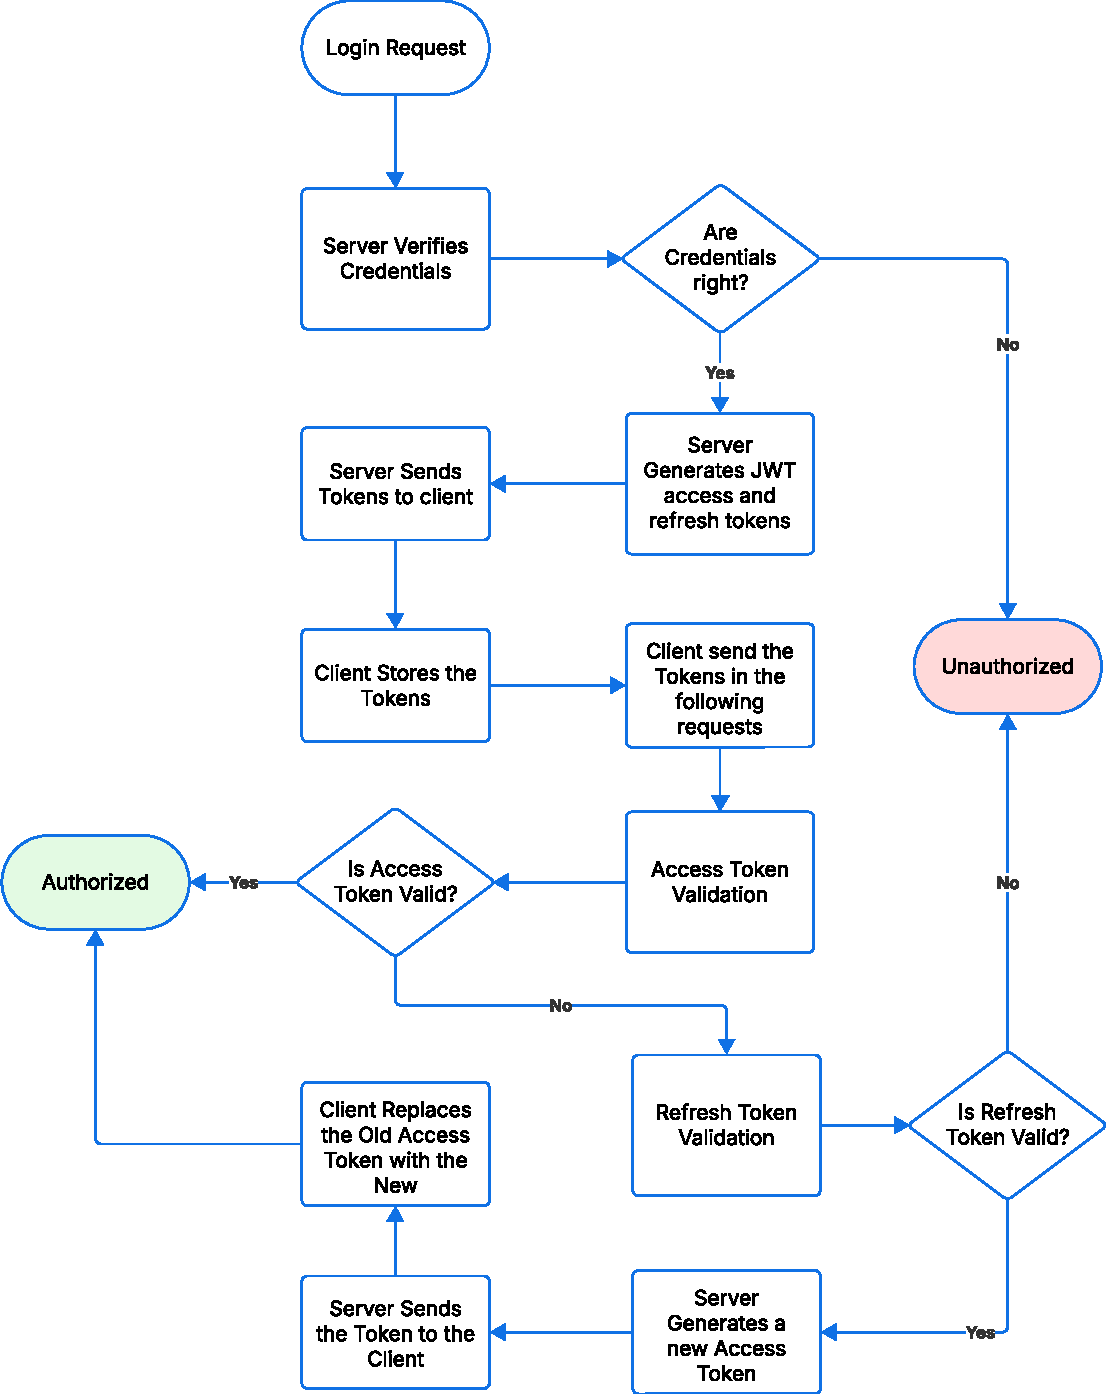
\includegraphics[width=0.9\textwidth, height=0.6\textheight, keepaspectratio]{Chapters/Figures/Security/JWT.pdf}
	\caption{Authentication process using JWT}
	\label{fig:security:JWT}
\end{figure}

\begin{itemize}

	\item \textbf{Authentication}

	      It's important that the component that does the request identifies itself
	      in a way that the other part can authenticate.
	      In the case of IoT to backend communication, IoT devices must authenticate
	      using approachs like token-based or certificate-based authentication.

	      In frontend to backend communication the most common approachs to
	      authentication are sessions and token-based authentication using JWT.
	      Figure \ref{} is a flow chart of the authentication process using JWT.
	      Firstly the server verifies the credentials, if the credentials are
	      correct, the server issues two tokens, an access token and a refresh
	      token. These tokens are stored in the client and send in all of the
	      following request to the server. The access token is used to validate
	      the access and has a short life span (usually around 15 minutes). When
	      the access token expires, the refresh token is used to generate a new
	      access token. The refresh token is valid for a longer period of time (
	      tipically one week).

	\item \textbf{Data Encryption}

	      The data can be encrypted during transmission with protocols like TLS/SSL.
	      These protocols ensure that data is only readable by the intended parts.
	      For frontend-backend communication, this can be achieved using the HTTPS
	      protocol.

	      For more sensitive applications, end-to-end ecryption can be used.

	\item \textbf{Data Integrity}

	      To ensure that data isn't changed during transmition, techniques like
	      HMAC can be used.

	\item \textbf{Access Control}

	      Some data may be restricted to a specific group of users, therefore the
	      system needs to check if the user that requests the data has
	      authorization to get that data. Techniques like RBAC can be used to
	      prevent access to sensitive data from users that can't access it.

	      In the frontend-backend communication, CORS policies can be used to
	      restrict which origins can access the backend API.

	\item \textbf{Preventing Attacks}

	      Lastly, attacks like XSS, SQL Injection or DoS need to be prevented.
	      In IoT systems, the firmware must be updated regularly to prevent this
	      attacks.
	      CSP can be used to prevent XSS attacks. For DoS, it's possible to enforce
	      rate limits and API quotas. To prevent SQL Injection, strategies like
	      input sanitization or the use of an ORM are essencial.
\end{itemize}

\subsubsection{GDPR/LGPD compliance}


\section{Database}
The storage and management of data, is an essencial part of IoT platforms.
Due to the high volume of data, the high frequency and the diversity of the
data, the effective design of a database is essencial to ensure query efficiency
and scalability.
IoT platforms generate diverse data types:
\begin{itemize}
	\item transactional metadata (e.g. device  IDs, user permissions)
	\item logs (e.g. event triggers)
	\item high-frequency time-series data (e.g. sensor measurements).
\end{itemize}

This section addresses the different types of databases, its advantages and
challenges in the context of IoT systems.

\subsection{Relational Databases (SQL)}
Relational databases organize data into tables with predefined schemas.
This tables can have relationships of one to one, one to many, or many to many,
defined using primary and foreign keys. Their transactions follow the ACID
(Atomicity, Consistency, Isolation, Durability) properties, ensuring data
consistency, integrity and reliability. Additionally, they provide a way of
doing complex querying, through a query language called \gls{SQL}, making them
a realiable choice for structured data requiring ACID compliance. The figure
\ref{fig:databases:sql}
is an example of an entity relationship diagram for a simple SQL database structure.
This diagram has a customer table, an order table, a product table, a product
category table and an additional table that handles the many-to-many
relationship between orders and products.


\begin{figure}[H]
	\centering
	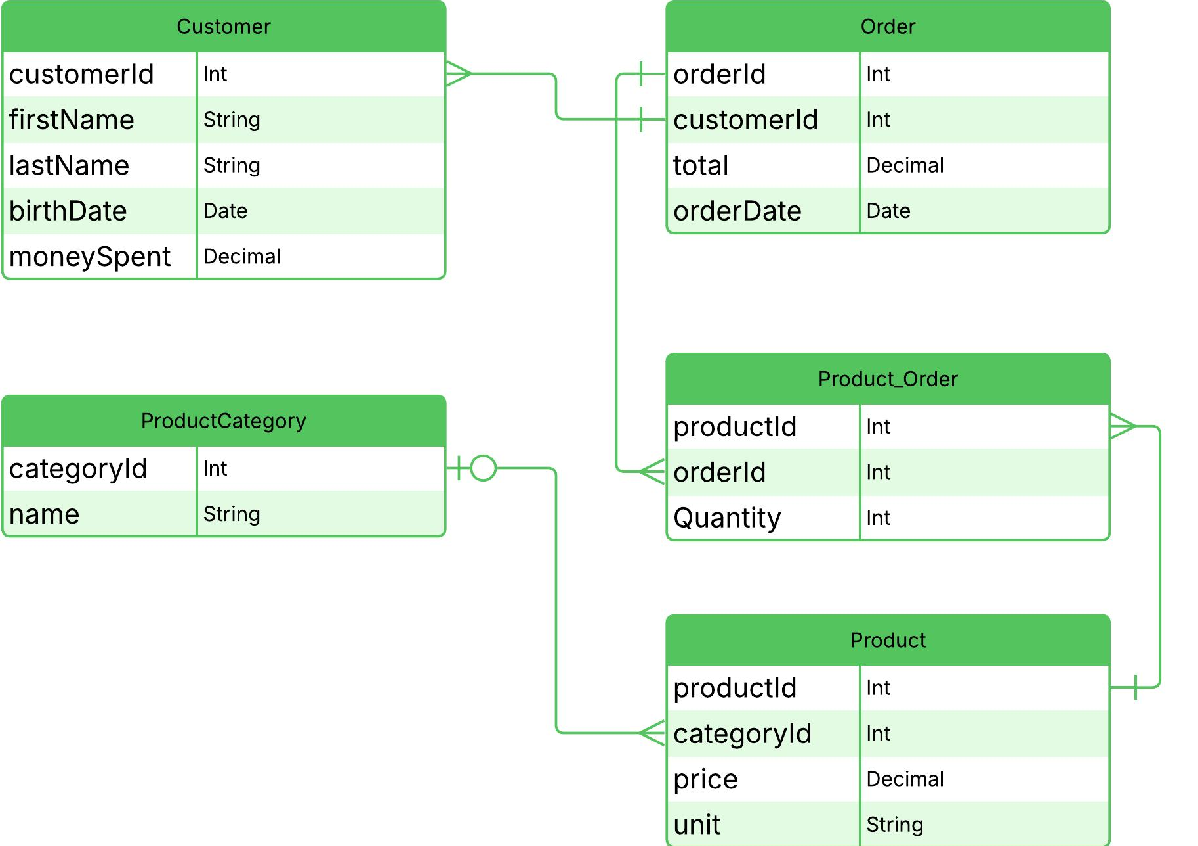
\includegraphics[width=0.9\textwidth, height=0.5\textheight, keepaspectratio]{Chapters/Figures/Databases/SQL.pdf}
	\caption{Example of a simple relational database entity relationship diagram. }
	\label{fig:databases:sql}
\end{figure}
\subsubsection{Advantages}

\begin{itemize}
	\item \textbf{Data integrity}

	      It allows the use of constraints (e.g. unique values, not null values,
	      foreign keys) to force strict rules, preventing anomalies and ensuring
	      reliability.

	\item \textbf{Complex Queries}

	      The use of SQL as a standard language allows complex queries with JOIN
	      operations and nested queries for relational data analysis.

	\item \textbf{Maturity}

	      There are already robust tools for backup, replication and access
	      control(e.g. PostgreSQL, MySQL).

\end{itemize}

\subsubsection{Challenges}
\begin{itemize}

	\item \textbf{Scalability}

	      Since IoT systems can generate a high amount of data, vertical scaling can
	      be costly.

	      In terms of horizontal scaling, traditional relational databases generally
	      struggle with adding more servers. Sharding is a popular approach to
	      solve this problem by spliting large tables into smaller segments(shards)
	      and store them in different servers, but it adds complexity to joins
	      across multiple shards.

	\item \textbf{Schema Rigidity}

	      In relational databases, tables follow a strict predefined schema, which
	      difficults the process of integrating new data types, like unstructured
	      data or new IoT devices.

\end{itemize}


\subsection{NoSQL Databases}
Not Only SQL (NoSQL) databases provide flexible schemas, making them suitable
for storing unstructured and semi-structured data. Following the CAP theorem,
NoSQL databases, unlike relational ones, prioritize availability and partition
tolerance over consistency. There are several types of NoSQL databases:

\begin{description}

	\item[Document Databases: ]Store data as JSON, BSON, or XML documents (e.g.
	      MongoDB, CouchDB, Firebase Firestore). Figure \ref{fig:databases:NoSQL}
	      shows an example of a JSON-like document that represents an order's data.
	\item[Column Oriented Databases: ]Store data in columns instead of rows (e.g.
	      Apache Cassandra, HBase, ScyllaDB).
	\item[Key-value Databases: ]Store data as key-value pairs, similar to
	      a hash table, providing fast access to data. Mainly used as cache. Some
	      examples include Redis and Amazon DynamoDB.
	\item[Graph Databases: ]Store relationships between entities as nodes and
	      edges. Popular databases include Neo4j, ArangoDB and Amazon Neptune.

\end{description}

\begin{figure}[htbp]
	\centering
	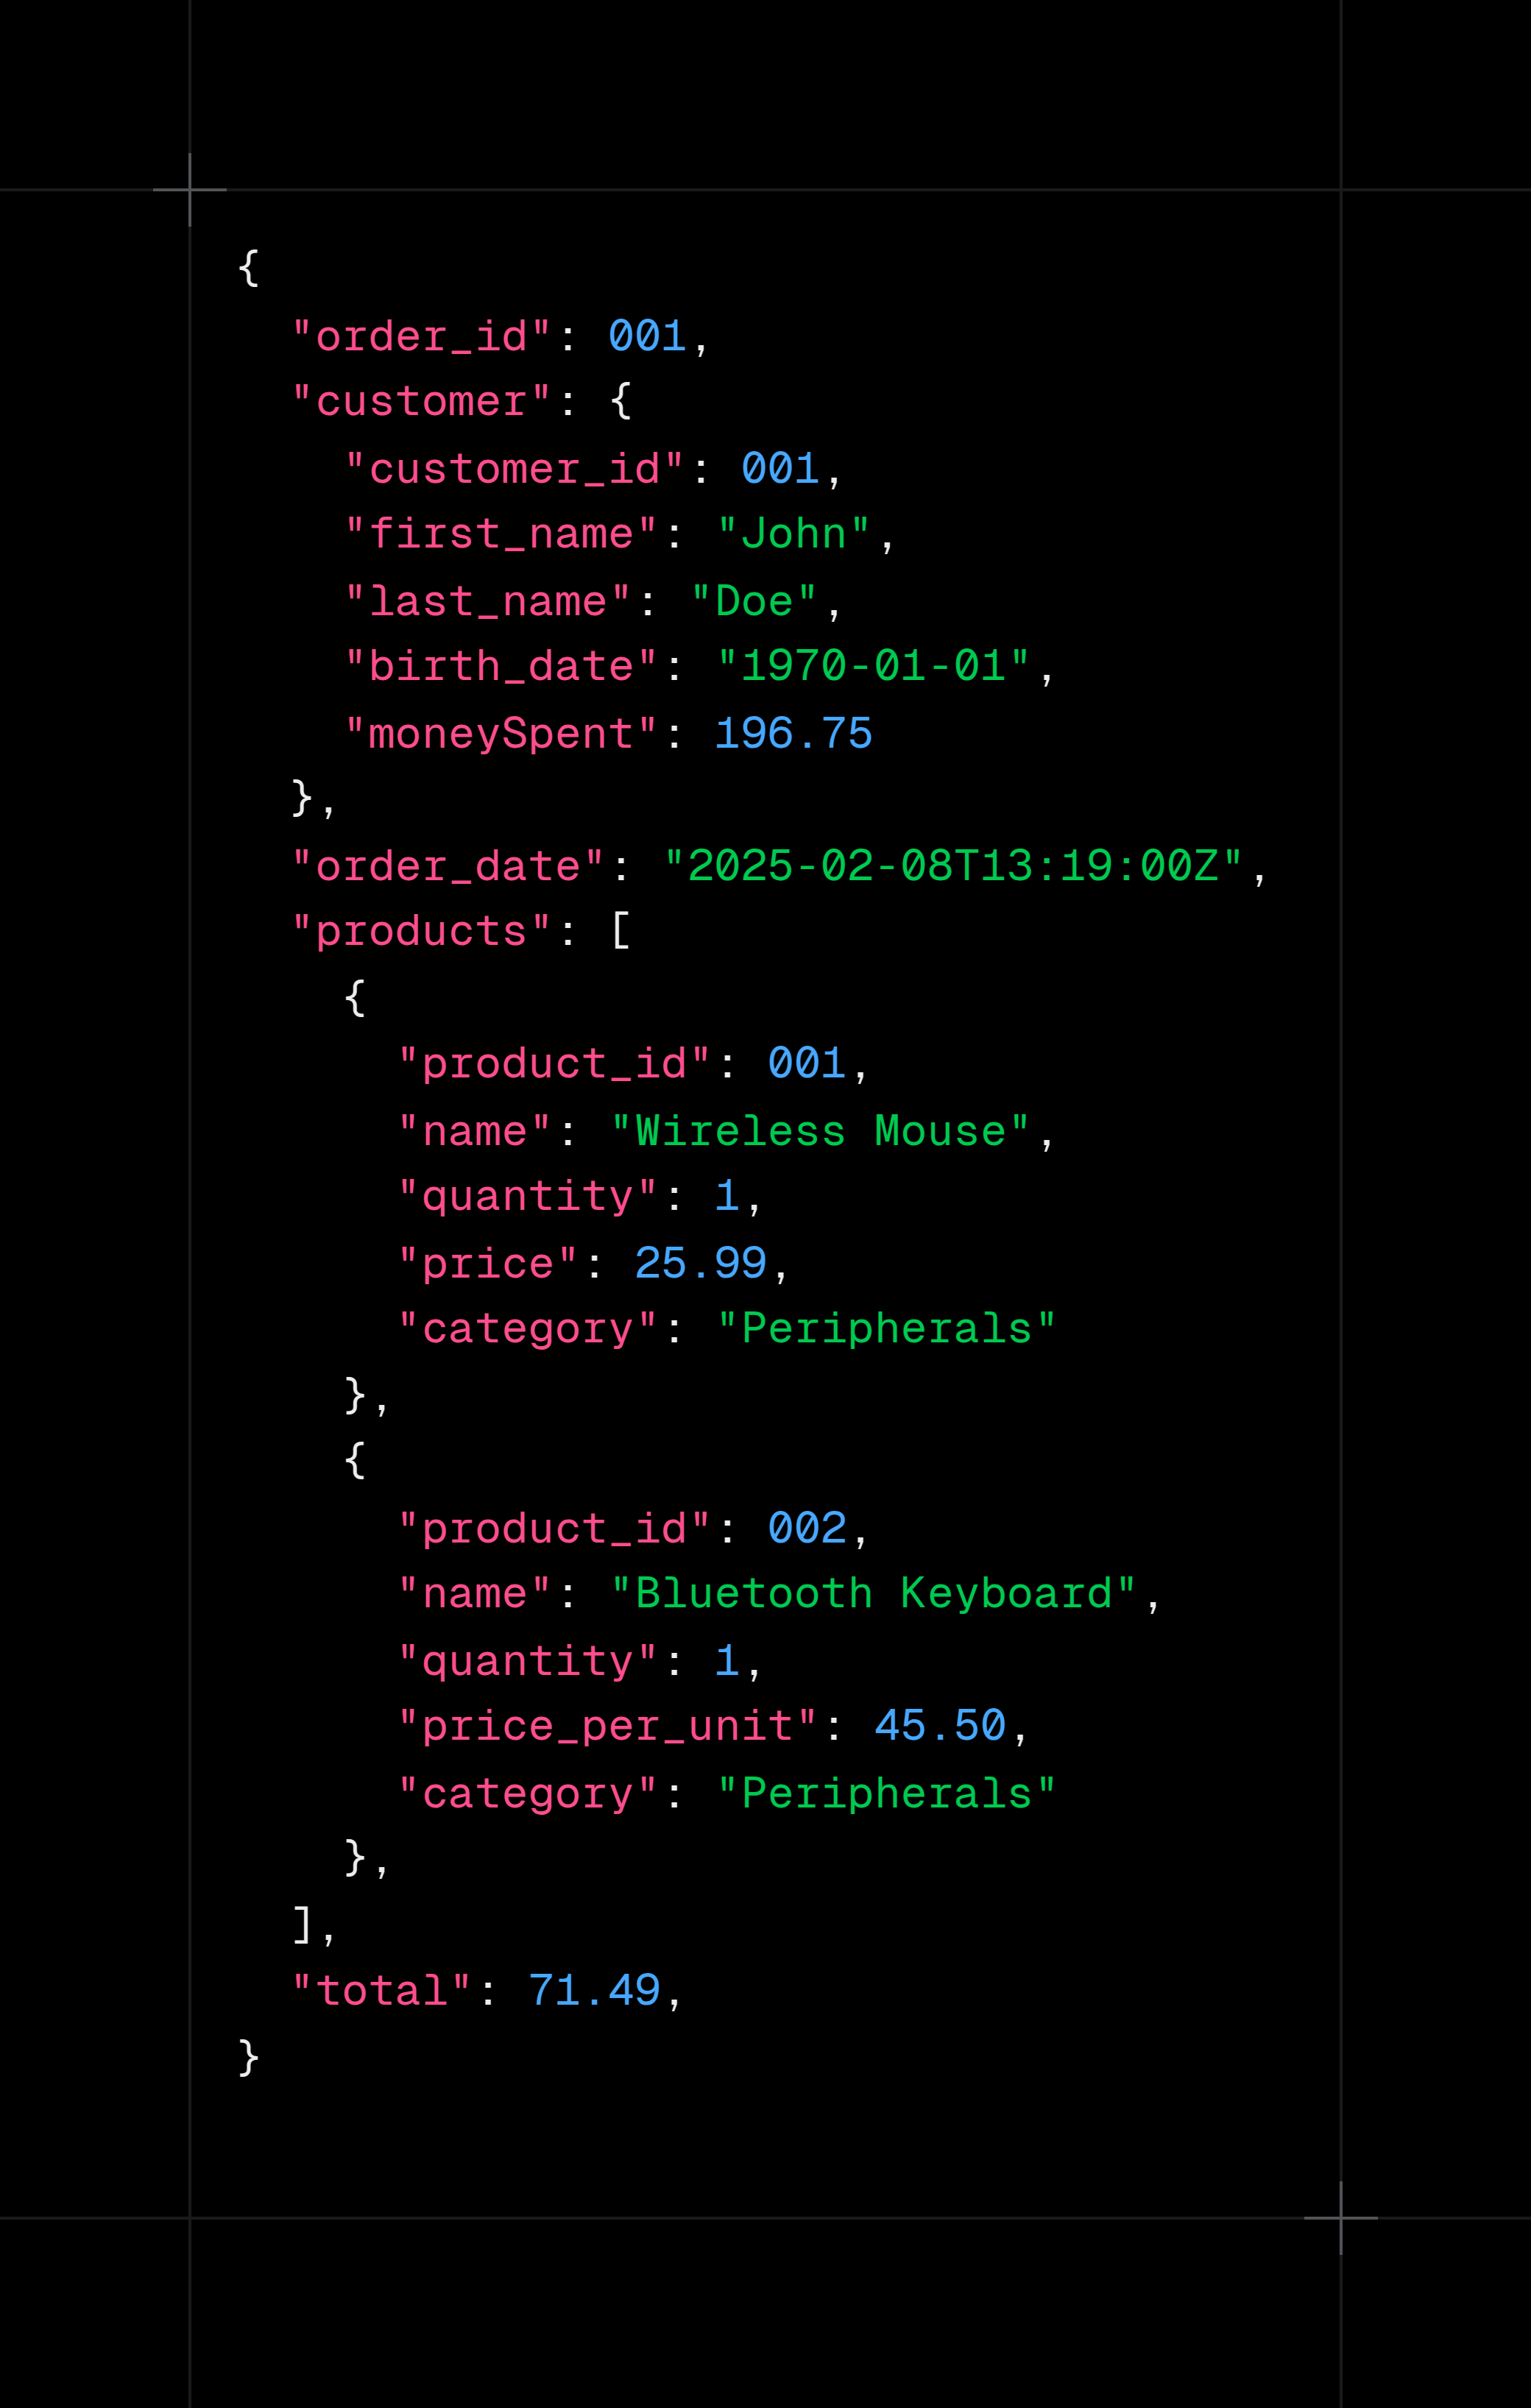
\includegraphics[width=0.9\textwidth, height=0.5\textheight, keepaspectratio]{Chapters/Figures/Databases/NoSQL.png}
	\caption{Example of a document-based database's JSON-like order document.}
	\label{fig:databases:NoSQL}
\end{figure}

\subsubsection{Advantages}
\begin{itemize}

	\item \textbf{scalability}

	      NoSQL Databases scale easily horizontally by spliting data across
	      multiple servers or clusters.

	\item \textbf{Performance}

	      NoSQL databases are optimized for speed and its transactions typically have
	      low latency. Due to its data being stored in an unstructured and simpler,
	      without constraints or relations, NoSQL databases operations are generally
	      faster when compared to relational databases. On top of this, many non
	      relational solutions implement in-memory storage, caching and efficient
	      indexing techniques, improving the performance even more.

	\item \textbf{Flexibility}

	      Unlike SQL databases that restrict the data to predefined rigid schemas,
	      NoSQL databases allow for dynamic schema changes, meaning that fields can
	      be added or removed to the schema on the fly without requiring database
	      migrations or even downtime.

	\item \textbf{Availability}

	      Many NoSQL solutions offer built-in replication and fault tolerance
	      technologies to ensure availability and fault tolerance. Typically data is
	      replicated across multiple nodes, so in case one node fails, the others
	      are up and have the data required.

\end{itemize}

\subsubsection{Challenges}

\begin{itemize}
	\item \textbf{Consistency}

	      According to the CAP theorem, database systems can only guarantee two out of
	      Consistency, Availability and Partition Tolerance. NoSQL Databases focus on
	      Availability and Partition Tolerance, leaving consistency to second plan.
	      This results in eventual consistency, meaning that data takes time to update
	      between nodes, leading to inconsistency in the meantime and leading to
	      consistency in the end.

	\item \textbf{Limited Query Capabilities}

	      NoSQL databases don't support complex queries with features like JOINs,
	      aggregations etc. making querying less flexible. Some databases have query
	      languages like SQL but even those are not as powerful as SQL queries.

	\item \textbf{Data Duplication}

	      In order to improve reading performance, some data is replicated across
	      multiple documents or collections, increasing storage requirements, and
	      making consistency harder to maintain.
\end{itemize}
\subsection{Time-Series Databases}
Time-series databases (TSDBs) are focused on storing time-stamped data. The
data is indexed by timestamp, making time-based queries very efficient. They are
optimized for high-velocity writes, making these databases a reliable solution
for storing sensor data on IoT systems. Popular time-series databases include
InfluxDB, TimescaleDB, and Prometheus.

\subsubsection{Advantages}
\begin{itemize}
	\item \textbf{High Write Throughput}

	      These databases are optimized for receiving millions of timestamped data
	      per second.

	\item \textbf{Efficient Querying}

	      TSDBs are optimized for querying and aggregating based on timestamps. This
	      makes real-time analytics efficient.

	\item \textbf{Edge computing compatibility}

	      Some lighter TSDBs like QuestDB can run on resource-constrained environments,
	      making possible to use this databases to store sensor data on the devices,
	      to be processed on the edger and then sent to the backend service.

\end{itemize}
\subsubsection{Challenges}

\begin{itemize}

	\item \textbf{Flexibility}

	      Despite being efficient with time-series data, it struggles with non
	      time-stamped data (e.g. user metadata). It is also not suitable for applications requiring
	      complex joins or relational data models.

	\item \textbf{High Storage Requirements}

	      Due to the high-speed of incoming data, it requires a high volume of storage
	      capacity. Strategies like data compression, prunning or retention policies
	      are essencial to the reduction of this problem.

\end{itemize}
\subsection{Applications and Use Cases}
Choosing the right databases to use is an important part of system design. This
choice must have into account the system requirements. Relational databases are
ideal when the system requires ACID compliance. It's also a good choice for
data that requires a rigid structure, constraints or relies heavily on
relationships between data. NoSQL databases are mostly used for unstructured
data, where flexibility is a crucial requirement.

In many cases, the best choice is an hybrid approach with different databases
being used for different types of data.

IoT systems rely on several kinds of data that differs a lot from each other.

Structure data like device metadata, or user metadata for accessing the
frontend pages would be better stored in relational databases for assuring
consistency. The constraints possible in SQL also ensures that the data is valid,
and structured. Lastly, queries that rely on relationships, for example finding
which sensors a user has access to are also easier on relational databases.

For data like sensor readings, which is unstructured and deeply associated with
the sensor reading time, time-series databases are a better choice. This data
is usually generated at a very high frequency, and time-series databases are
optimized for high-speed writing. Real-time data processing is also better with
this databases, because despite time-based queries being possible and common in
relational databases, they are optimized in time-series databases, making
real-time analytics more efficient.

NoSQL, more precisely, document or column oriented databases, in IoT systems
context, can also be a great choice for storing unstructured data that isn't
time-based, for example events spoted from analyzing sensor data.

Lastly, for the web application, key-value databases like redis can be usefull
for caching, and relational databases can be used for handling for example
role-based access.

\section{Frontend Development}
Frontend is the part of a web application that runs in the user's browser and
the part that the user can see and interact with. It is divided into three
parts: Markup, styling and scripting.
The markup defines the structure of the website, the styling is the part that
defines all of the styling of the page including colors fonts and empty spaces
(margins/paddings) and the scripting is the part that enables the interaction
of the user with the website, including buttons functionalities, form handling
etc..
It can be developed in many languages but all of them are in the end transpiled
to the languages that the browsers can understand which are: Hypertext markup
Language (HTML) for markup, Cascading Stylesheets (CSS) for styling and
Javascript (JS) for scripting.

\subsection{Frameworks and Libraries}
With the advance of technology many libraries were created to facilitate the
frontend development experience. This section addresses the most popular
frotend web development javascript libraries and frameworks.
\subsubsection{ReactJS}
React JS is an open-source javascript library created by Facebook in 2013 that
simplifies the development of complex and dynamic user interfaces. Its the most widely
used library of its kind.
React applications are build using components. Components are reusable pieces of
code that represent a part of the UI, e.g. a button, a form or an entire section.
Each component has its own logic and styling and its declarative i.e. the
component defines what the UI should look like for a given state.
Components can be nested inside other components to build more complex UIs.
The components are developed using JavaScript for scripting and JavScript XML(JSX),
which is similar to HTML for markup.

React uses a virtual Document Object Model (DOM) to optimize performance. A virtual
DOM is a lightweight in-memory representation of the real DOM, which is a
representation of the HTML structure in a tree-like structure. When a change
occur, it updates the virtual DOM first, then calculates the minimal changes needed
and then apply these changes to the real DOM\cite{bawane2022review}.

\subsubsection{NextJS}
NextJS is a full-stack framework built on top of reactJS by vercel. This means
that NextJS can be used to develop both the frontend and backend parts of the
web application. Besides that, NextJS has several more advantages on ReactJS
adding features such as file-system based routing, server-side rendering (SSR)
and automatic code splitting.

One of Reactjs problems is that it doesn\'t have built-in support for routing,
meaning that the page routing needed to be handled using third party libraries
like react-router-dom. NextJS solves this issue by having a file-system based
routing. This works by automatically mapping every page file (a JSX/JS/TSX/TS
file named page) to an URL. This url is defined by the path of that file
relative to the app folder, which means that a file in app/report/test/page.tsx
is mapped to the endpoint report/test.

Another improvement of NextJS relative to ReactJS is that it allows SSR. In
Client Side Rendering, used by react, the server sends to the server a small
html document and a link to the javascript which the client needs to download
and run. On the other side, with SSR, the server sends to the browser the
full HTML document which it just needs to render\cite{Salanke_A.R_G.S_Dalali_2022}.

Apart from the clear performance increase, the SSR also improves the Search
Engine Optimization. This happens because the search engine scans the static
html page, and doesn\'t have into account the dynamic html created after by
the script. SEO can also be improved in another way, through the website
metadata (title, description, keyworks etc..) which NextJS also makes easier to
manage because of its ready-to-use Head component.

Another feature that improves the performance of projects using this framework
is the automatic code splitting. The automatic code splitting consists in
the separation of the javascript bundle into small parts that can be loaded
separately. This reduces significantly the page load time, by loading only the
parts that are needed to display the requested page.

\subsubsection{Angular}
Angular is a typescript based, open-source framework used for building user
interfaces. It was developed by Google in 2016 as a new, restructured version
of AngularJS. Angular is a strongly structured and opinionated framework,
organizing the code into feature modules. It also follows a component-based
design, but introduces features like dependency injection ensuring efficient
state sharing and improving testability.
It includes built-in features like routing, HTTP client and form validation.

\subsection{State Management}
State management is a fundamental aspect of frontend development. It enhances
the user experience providing data consistency and an improved performance.
State represents the dynamic data of an application an can be of three types:

\begin{description}

	\item[Local state:] The state managed within a single component. It can
	      represent data from UI elements like forms or button states.

	\item[Shared state:] When multiple components need access to the same data,
	      that data can be shared between them using solutions like context APIs or
	      external libraries.

	\item[Global state:] Usually used for user authentication, notifications and
	      data persistance, the global state is application-wide, meaning that
	      every component has access to it.
\end{description}

Handling global state is a complex proccess and requires the use of state
management solutions like Redux, Recoil, Zustand, or Jotai for ReactJS and
NgRx, Elf or NGXS for Angular.

\section{Data Processing Pipelines}
A data processing pipeline is a structured workflow that transforms raw data
into usefull insights. These pipelines are essential for handling an high-volume
of data in real-time. Data pipelines must ensure scalability, fault tolerance,
efficiency, data quality and real-time processing.

\subsection{ETL for IoT}
\gls{ETL} is a workflow that transforms raw data into data that is ready for
store. IoT systems use \gls{ETL} pipelines to process and store data from sensors,
smart devices, and edge computing nodes. Figure \ref{fig:etl:pipeline}
ilustrates the \gls{ETL} pipeline, with the data being extracted from de devices,
transformed and then loaded to the database.

\begin{figure}[htbp]
	\centering
	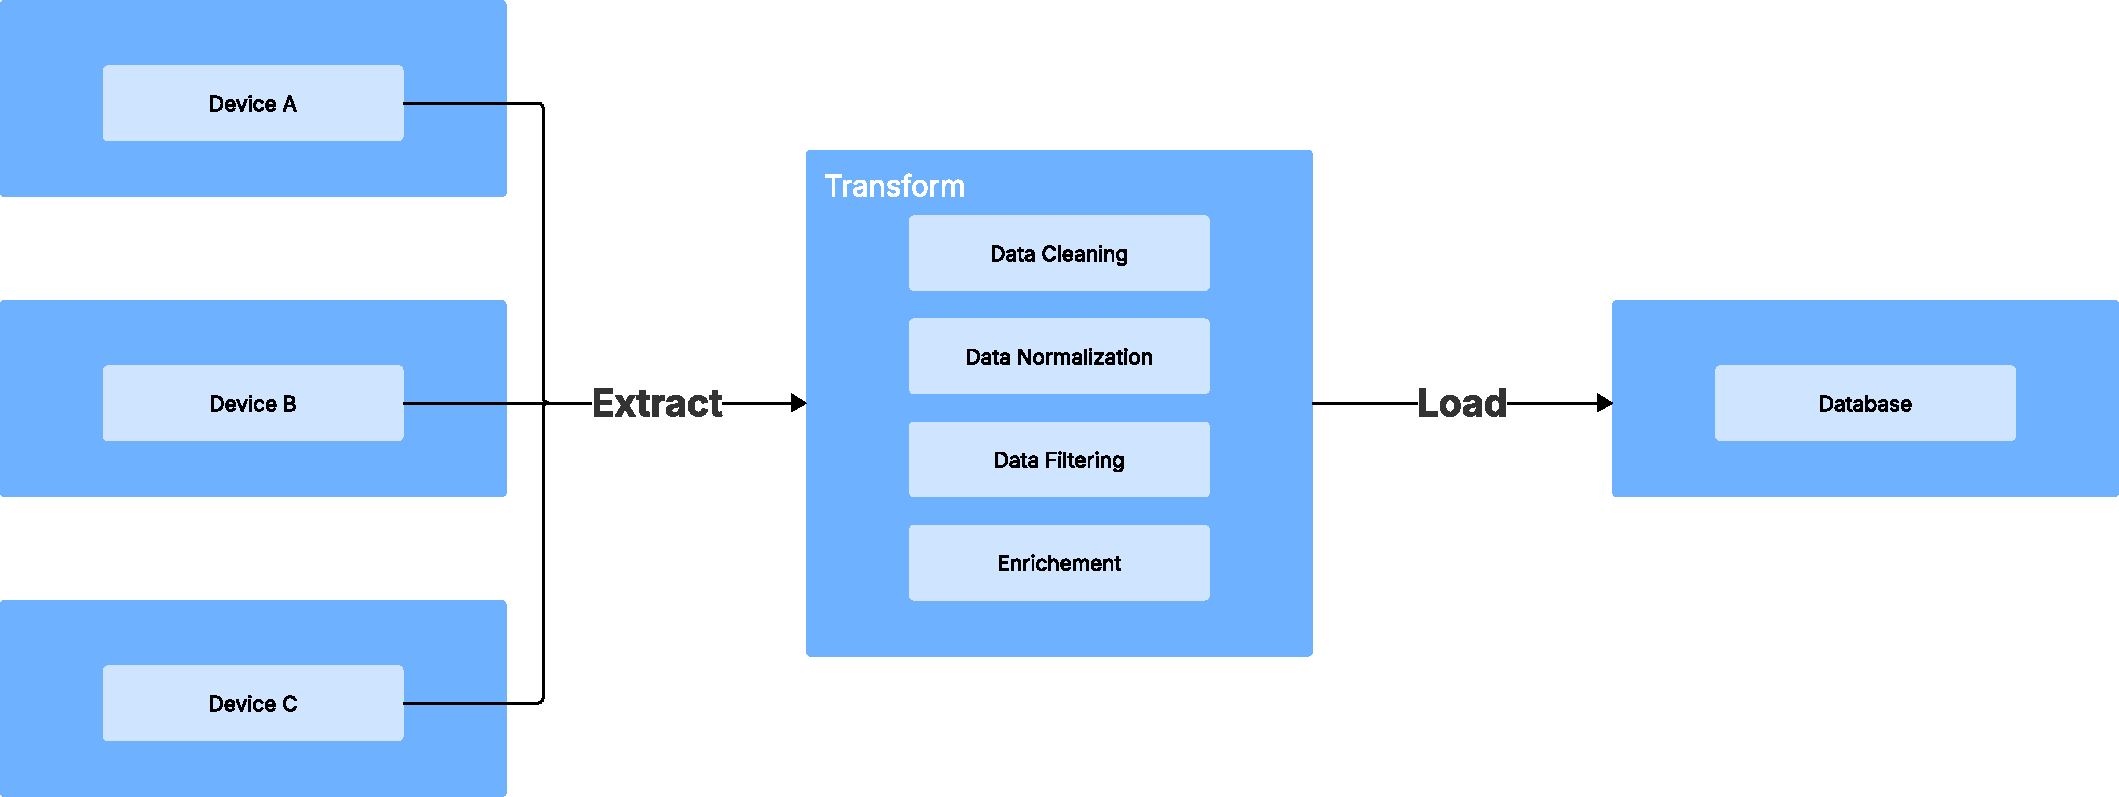
\includegraphics[width=0.8\textwidth, height=0.5\textheight, keepaspectratio]{Chapters/Figures/ETL/ETL.pdf}
	\caption{ETL Pipeline.}
	\label{fig:etl:pipeline}
\end{figure}

\subsubsection{Extract}
The first step is the extraction. In this step, the raw data is collected from
IoT devices, APIs, cloud platforms or edge systems. This can be done through
MQTT brokers, HTTP or CoAP endpoints, Apache Kafka streams or IoT gateways.

\subsubsection{Transform}
The extracted data is then transformed through a sequence of processes. These
processes, among others, include cleaning, filtering, and enriching.
In the first, the data is cleaned, filtering noise, removing duplicates, and
null values. In the filtering, the data is filtered, discarding irrelevant data
for the purpose. For example, if the purpose is to use a temperature sensor to
check for high temperatures, this process discards all the data that is
considered a normal temperature. The data can also be enriched with metadata
like timestamps, device location, etc. This stage can be done on the edge, on
the cloud or using an hybrid approach. There are cloud tools like Apache NiFi
and AWS IoT Analytics designed for transforming data.

\subsubsection{Load}
Load is the stage in which the transformed data is stored in databases.

\subsection{Business Intelligence}
\gls{BI} refers to the strategies, technologies and tools used to process and
analyze raw data for decision-making, monitoring and strategic planning.
This data can be shown through data visualization tools, and analytics.
In IoT systems, \gls{BI} tools are essencial to understand trends, detect
anomalies and optimize operations.

The data visualization can be done through dashboards, for monitoring real-time
metrics, geospatial maps, for visualization of devices or anomalies locations,
or customized reporting for regulatory compliance or audits. The analytics, can
be of several types: descriptive, diagnostic, predictive, prescriptive and
real-time analytics. Descriptive analytics are used to summarize historical
data, diagnostic analytics are for finding the cause of specific problems, and
predictive analytics use machine learning algorightms to predict future events.
Prescriptive analytics use the predictions generated by predictive to recommend
actions, and lastly, real-time analytics process data in real-time to make
decisions instantly.

There are many \gls{BI} visualization tools available for integration with IoT systems.
Tableau, Microsoft PowerBI, Looker and Grafana are some of the most popular ones.

To make analytics easier, there are several ready-to-use tools for generating
analytics from raw data. Examples include Apache Flink, Apache Spark,
TensorFlow and ElasticSearch.
\subsubsection{Challenges}

\begin{itemize}
	\item \textbf{High Cost}

	      Due to the high volume of data, an high-performance and high capacity storage
	      solution is required, which increases the cost significantly. On top of this,
	      licences for \gls{BI} tools are expensive and free tools are usually very
	      limited in terms of features.

	\item \textbf{Data Consistency}

	      Ensuring consistency between data from different sources can be difficult.
	      The data preparation can be a complex process and an efficient \gls{ETL} is
	      essencial to prevent inconsistencies.

\end{itemize}


\section{AI/ML for Anomaly Detection}
Anomaly detection is the process of identifying data that deviates from the norm.
In IoT systems, anomalies can represent equipment failures, traffic violations,
security breaches etc. Machine learning and artificial intelligence techniques
can be integrated in the data process pipeline to detect anomalies.



\subsection{Frameworks}
\begin{table}[ht]
	\centering
	\caption{Comparison of AI/ML Frameworks for Anomaly Detection}
	\label{tab:ai-ml:frameworks}
	\begin{tabular}{p{2cm}p{4cm}cp{3cm}}
		\toprule
		\textbf{Framework} & \textbf{Key Features}                  & \textbf{Edge Support} & \textbf{Use Cases}             \\
		\midrule
		TensorFlow         & Deep learning, TF Lite for edge        & Yes                   & Time-series, Image recognition \\
		PyTorch            & Dynamic graphs, research-friendly      & Partial               & Custom models, Research        \\
		Scikit-learn       & Classical ML (e.g., SVM)               & No                    & Structured data analysis       \\
		Prophet            & Time-series forecasting                & No                    & Predictive maintenance         \\
		Edge Impulse       & Edge-first ML, microcontroller support & Yes                   & Real-time edge inference       \\
		\bottomrule
	\end{tabular}
\end{table}

Machine learning frameworks are essential for designing and training machine
learning models. The table \ref{tab:ai-ml:frameworks}
compares some of the most popular frameworks in IoT context.

\subsection{Deployment}

\subsection{Challenges}

\begin{itemize}
	\item \textbf{Data Imbalance}

	      Anomalies are rare, and synthetic data generation may be needed to train
	      the model.
	\item \textbf{Cold Start}

	      In the beginning, there's a low amount of data to train the model.
	\item \textbf{Model Drift}

	      Sensor behaviour changes over time.
\end{itemize}

\section{Related Work}
